% Sample apostrophy's to remove team's 

\chapter{Research Method}
\label{ResearchMethodChapter}
\label{ResearchMethod}


\section{Constructivist Grounded Theory}

When deciding which version of Grounded Theory to employ, we selected Constructivist Grounded Theory \cite{Charmaz} because it allows for the recording and transcription of interviews, enables literature review when appropriate in the research process, and builds upon decades of grounded theory research and experience.

The philosophical stance of constructivism (as opposed to positivism) acknowledges the reseacher's and participants' contribution in the construction of concepts. 
While there are absolute facts to be obtained in fields such as mathematics and the sciences, understanding people is a messy, organic process. For software engineering research, Constructivist Grounded Theory seems aptly suited since software development is a socio-technical endeavor.

As described in Chapter \ref{ConstructivistGroundedTheoryChapter}, Constructivist Grounded Theory provides an iterative approach to data collection, data coding, and analysis resulting in an emergent theory. Grounded Theory research begins by asking, \quotes{what is happening here?} \cite{GlaserTheoreticalSensitivity}; or in this case, \quotes{what is happening at Pivotal when it comes to software development?} 

In time, \quotes{team code ownership} and \quotes{removing waste} emerged as two of the core categories. Exploring theoretical saturation for team code ownership resulted in the theory of sustainable software development presented in Chapter \ref{SustainableSoftwareDevelopmentChapter} and five factors that affect a team's sense of code ownership presented in Chapter \ref{TeamCodeOwnershipChapter}. Exploring theoretical saturation for removing waste resulted in a taxonomy of software  engineering waste presented in Chapter \ref{SoftwareEngineeringWasteChapter}.

\section{Research Context: Pivotal Labs}
\label{SustainableSoftwareDevelopmentResearchContext}

Pivotal Labs is a division of Pivotal\textemdash a large American software company (with 17 offices around the world). Pivotal Labs provides teams of agile developers, product managers, and interaction designers to other firms. Its mission is not only to deliver highly-crafted software products but also to help transform clients' engineering cultures. To change the client's development process, Pivotal combines the client's software engineers with Pivotal's engineers at a Pivotal office where they can experience Extreme Programming \cite{BeckExtremeProgramming2004} in an environment conducive to agile development. 

Typical teams include six developers, one interaction designer, and a product manager. The largest project in the history of the Palo Alto office had 28 developers while the smallest had two. Larger projects are organized into smaller coordinating teams with one product manager per team and one or two interaction designers per team.

Interaction designers identify user needs predominately through user interviews; create and validate user experience with mockups; determine the visual design of a product; and support engineering during implementation. Product managers are responsible for identifying and prioritizing features, converting features into stories, prioritizing stories in a backlog, and communicating the stories to the engineers. Software engineers implement the solution. 

Commonly utilized technologies include Angular, Android, backbone, iOS, Java, Rails, React, and Spring. These are often deployed onto Pivotal's Cloud Foundry. 

Pivotal Labs has followed Extreme Programming \cite{BeckExtremeProgramming2004} since the late 1990's. While each team autonomously decides what is best for each project, the company culture strongly suggests following all of the core practices of Extreme Programming, including pair programming, test-driven development, weekly retrospectives, daily stand-ups, a prioritized backlog, and team code ownership. Only  teams at Pivotal Labs were observed. Other teams, especially teams in other divisions, might have a different culture and follow different software practices.

Pivotal is an good research location because: 1) it is successful; 2) it is interesting in its continued use and evolution of extreme programming; 3) it is accessible and cooperative with research. Both Classic and Constructivist Grounded Theory advocate picking an interesting site to see \quotes{What's going on here?}

\section{Data Collection}
This research study analyses data from three sources: 1) interviews with Pivotal employees, 2) participant observation of \numberOfObservedProjects{} projects over \durationOfResearchStudyPlural{}, and 3) topics discussed in 91 retrospection meetings. 

For this grounded theory study, the two primary data sources were field notes collected during continuous participant observations of a seven-month project and interviews with Pivotal software engineers, interaction designers, and product managers.

\subsection{Interviews}
The interviewees consisted of \numberOfInterviews{} interaction designers, product managers, and software engineers who had experience with Pivotal's software development process from five different Pivotal offices. Interaction designers identify user needs predominately through user interviews; create and validate user experience with mockups; determine the visual design of a product; and support engineering during implementation. Product managers are responsible for identifying and prioritizing features, converting features into stories, prioritizing stories in a backlog, and communicating the stories to the engineers. Software engineers implement the solution. Participants were not paid for their time. 

We relied on \quotes{intensive interviews,} which are \quotes{open-ended yet directed, shaped yet emergent, and paced yet unrestricted} \cite{Charmaz}. Open-ended questions were used to enter into the participant's personal perspective within the context of the research question. The interviewer attempts to abandon assumptions to better understand and explore the interviewee's perspective. Charmaz \cite{Charmaz} contrasts intensive interviews with informational interviews (collecting facts), and investigative interviews (exposing hidden intentions, practices or policies).

The initial interviews were open-ended explorations starting with the question, \quotes{Please draw on this sheet of paper your view of Pivotal's software development process.} The interviewer specifically did not force initial topics and merely followed the path of the interviewee. 

While exploring new emergent core categories, whenever possible, subsequent interviews were initiated with open-ended questions.  For example, when team code ownership emerged as one of the core categories, asking the participant, \quotes{Please draw your feelings about the code} often resulted in conversations about code ownership. The interviews were spread across the duration of the research study. 


\subsection{Participant Observation}
We collected field notes while the lead researcher worked as an engineer on \numberOfObservedProjects{} projects. These notes describe individual and collective actions, capture what participants found interesting or problematic, and include anecdotes and observations.

Projects are de-identified to preserve client confidentiality:
\begin{itemize}
\item Project Unum (two product managers, four developers) was a greenfield project providing a web front end for installing, configuring, and using a multi-node cluster with big data tools. 
\item Project Duo (two interaction designers, two product managers, six developers) added features to a print-on-demand e-commerce platform. 
\item Project Tes (one interaction designer, one product manager, six developers) added features to management software for internet service providers.
\item Project Quattuor (two interaction designers, three product managers, 28 developers) developed two mobile applications and a backend system for controlling expensive equipment.
\item Project Kvin (one interaction designer, one product manager, six developers) was a greenfield project for a healthcare startup. 
\item Project Ses (two interaction designers, one product manager, ten developers) was adding features and removing technical debt to an existing internet e-commerce website.
\item Project Septem (two interaction designers, three product managers, twelve developers) was adding features and removing technical debt to an existing virtual machine management software.
\item Project Octo (one product manager, four developers) added features for workload management of a multi-node database.
\end{itemize}



\subsection{Retrospection Topics}
When \textit{removing waste} emerged as one of the core categories from interviews and participant observation, we began collecting data from retrospection meetings. A retrospection meeting (or retro) is a meeting to pause, reflect, and discuss the work done during the week, i.e., a safe place where any team member can discuss any issue \cite{DerbyAgileRetrospectives}. Retros are typically scheduled every Friday afternoon. The entire team and important stakeholders attend these meetings. 

The observed Pivotal teams mostly use an emotion-based retro format where \quotes{happy,} \quotes{neutral,} and \quotes{sad} faces are written on the top of a whiteboard. The happy-face column represents items that are working well and should be continued or expanded. The neutral-face column represents items that the team needs to \quotes{keep an eye on.} The sad-face column represents problems that the team should try to fix. Any team member can add any topic to any column. After a few minutes, the team dot-votes on the topics to discuss \cite{DerbyAgileRetrospectives}. The team uses the remainder of the sixty-minute meeting to discuss topics. Sometimes discussing a topic is sufficient to affect change, other times the team creates action items. 

We collected data from 91 retrospection meetings over 59 weeks from Projects Quattuor, Kvin, and Ses. (There are more meeting than weeks since each of Project Quattuor's three teams held its own retro each week.)


For co-located teams, a whiteboard picture was taken at the end of the retro and the topics were later transcribe into a master spreadsheet. For distributed teams, we copied data from the online spreadsheets the team used in place of a whiteboard. Attendees often wrote a short phrase as a proxy for a larger idea (e.g.,  \quotes{Scope} represents \quotes{Too much scope is causing the team stress}). When the provided topic was too vague, we solicited a more detailed description from an engineer that was present at the meeting. This produced 663 total items for analysis. 


\section{Data Analysis}
Data analysis began by iteratively collecting and analyzing interview transcripts and participant observations. We used line-by-line coding \cite{Charmaz} to identify nuanced interactions in the data and avoid jumping to conclusions. We reviewed the initial codes while reading the transcripts and listening to the audio recordings.  We discussed the coding during weekly research collaboration meetings. To avoid missing insights from these discussions \cite{GlaserTheoreticalSensitivity}, we recorded and transcribed them into grounded theory memos. As data was collected and coded, we stored initial codes in a spreadsheet and we used constant comparison to generate focused codes.

We routinely compared new codes to existing codes to refine codes and eventually generate categories. We periodically audited each category for cohesion by comparing its codes. When this became complex, we printed codes on index cards, and then arranged and re-arranged until cohesive categories emerged. We wrote memos to capture the analysis of codes, examinations of theoretical plausibility, and insights.

\begin{figure}[t]
\centering
\fbox{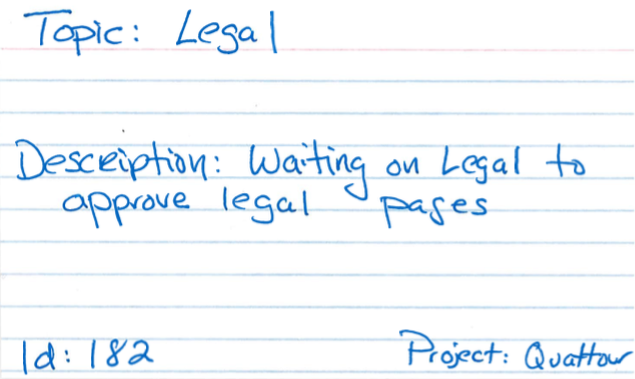
\includegraphics[width=3in]{waste_images/retro_index_card.png}}
\caption{Example Retro Topic Index Card}
\label{exampleRetroTopicl}
\end{figure}

 When \textit{removing waste} appeared as a core category, we analyzed data from retrospectives to investigate (theoretical sampling). After removing irrelevant topics (e.g. complaints about the weather), we printed each retro item onto an index card with its original retro topic, enhanced description, ID, and team name (see Figure \ref{exampleRetroTopicl}).

Two researchers with first-hand experience of the projects coded the retro topics and merged duplicate topics. We iteratively reorganized categories, keeping similar items together and dissimilar items apart. Figure \ref{ChainOfEvidence} gives an example classification for the \textit{psychological distress} waste. The figure shows the waste category, its cause categories and properties, and examples of observed retrospective topics illustrating the waste.  Appendix \ref{AppendixChainOfEvidence} presents the entire chain of evidence for all waste categories.

We often stopped to record new insights. When the categories began to stabilize, we compared each category against the other categories looking for relationships. Once we felt that the categories were stable, we performed a final review of each category to verify that the cards belonged to it.

We continued theoretical sampling for team code ownership and removing waste in additional interviews and participant observations until no further categories were evident, i.e. theoretical saturation. 

In summary, the data advanced from the initial codes to focused codes, focused codes to core categories, and core categories to an emergent theory. 


